\begin{appendices}

\chapter{Results from Evaluation} \label{appendix:results_table}
Contents of each run from the evaluation section where the second method is applied. 

\begin{figure}
\centering
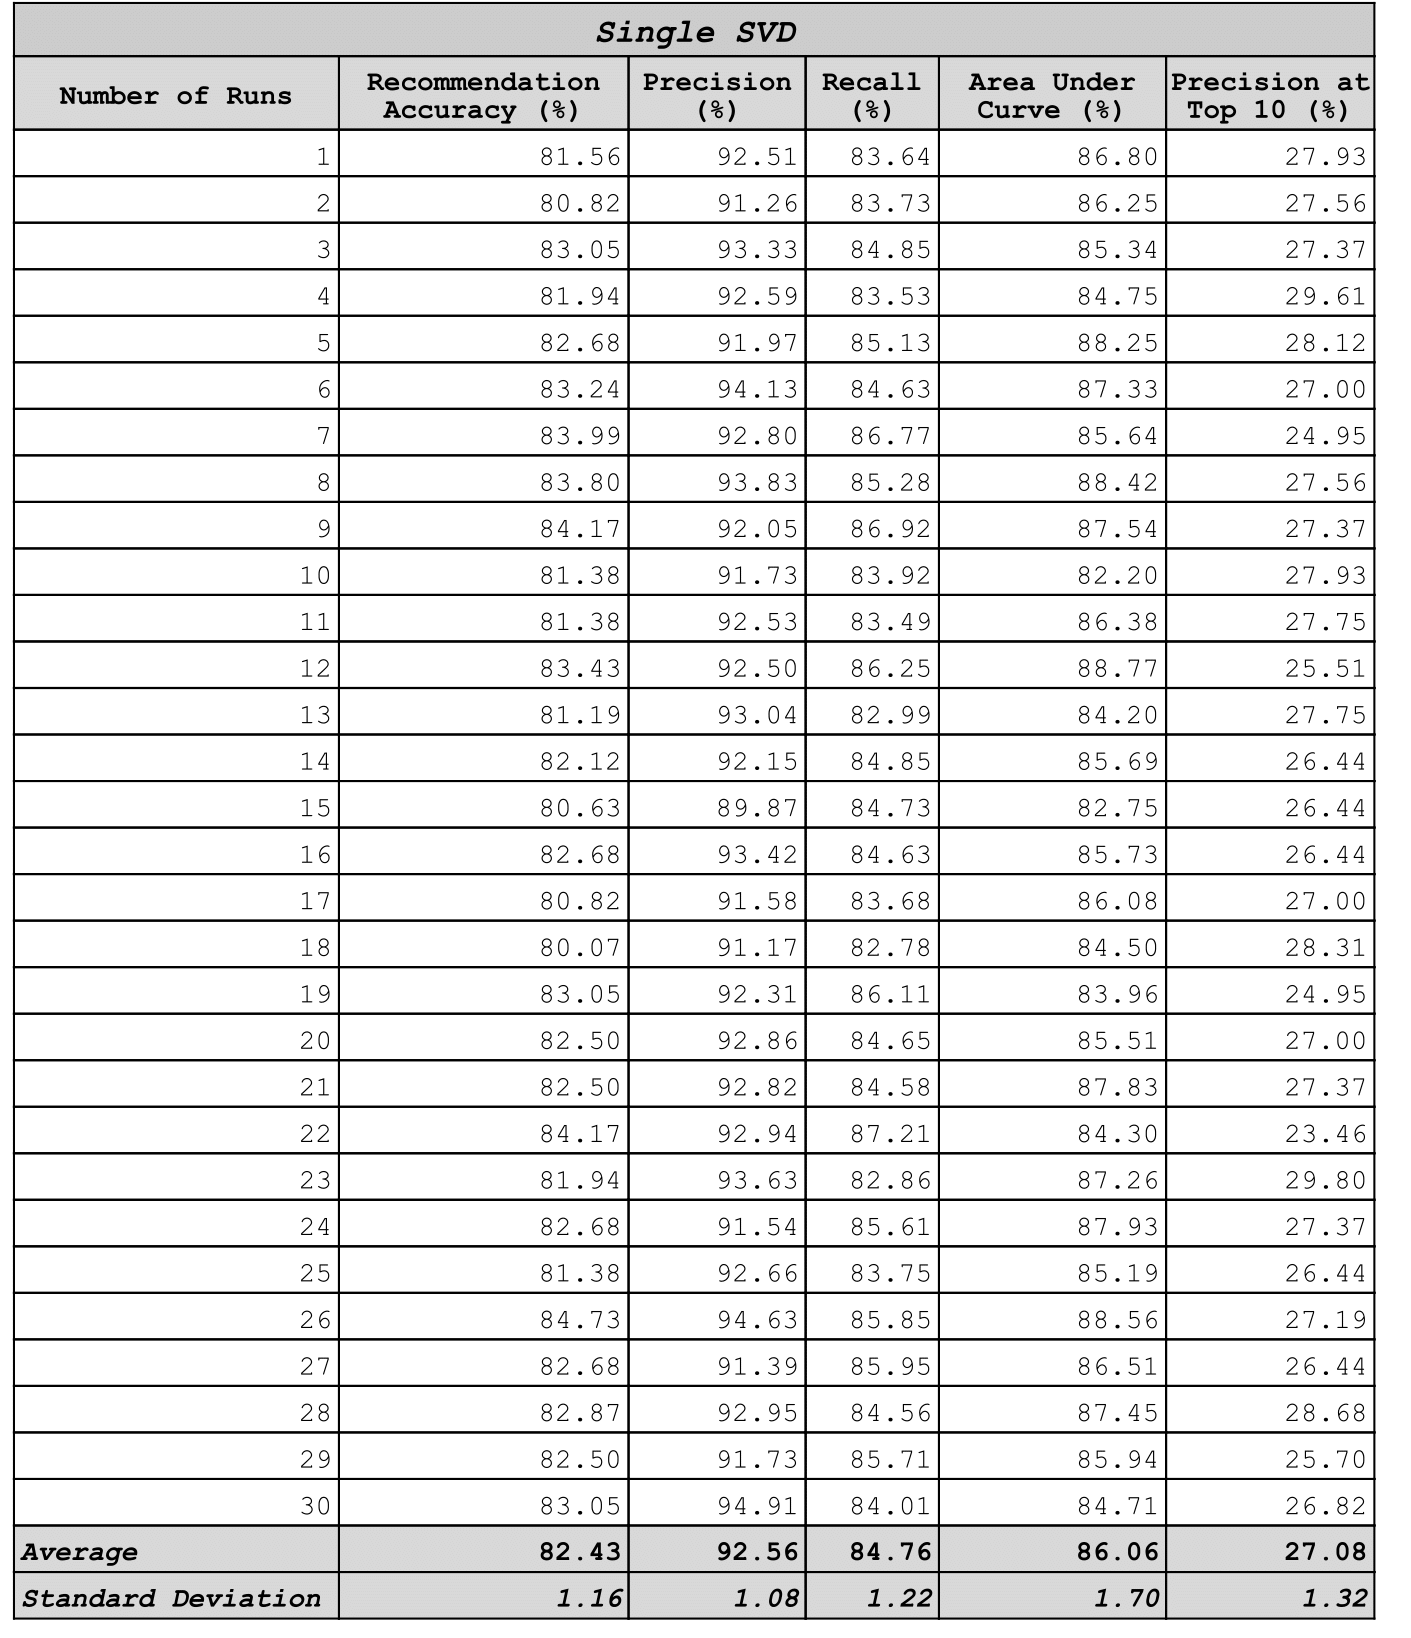
\includegraphics[scale=0.3]{appendices/single_als_30_runs.png}
\caption{Individual 30 runs of the Single SVD system.}
\label{fig:single_algorithm}
\end{figure}

\begin{figure}
\centering
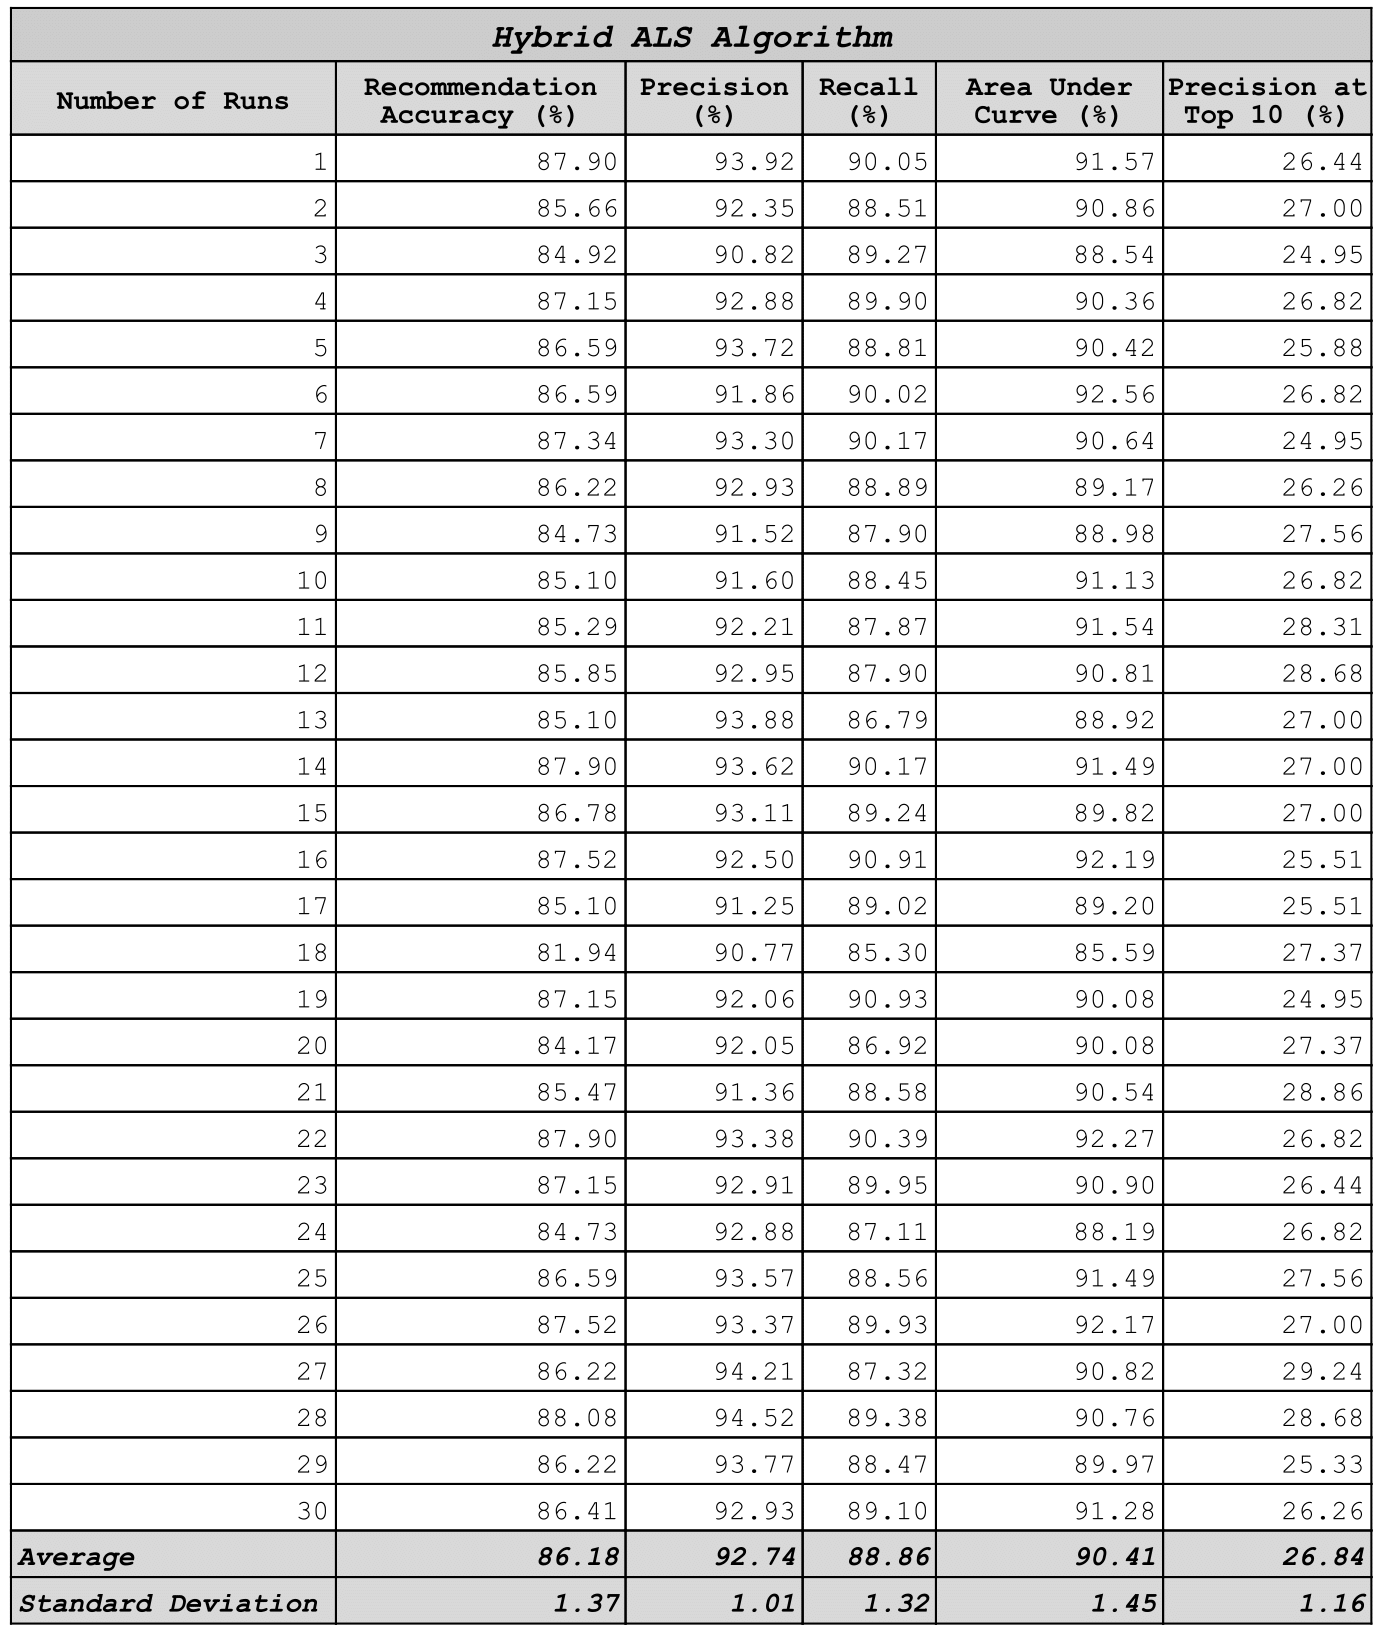
\includegraphics[scale=0.3]{appendices/hybrid_als_30_runs.png}
\caption{Individual 30 runs of the Hybrid SVD algorithm which takes into account the content preferences of the user and considers these preferences when making recommendations.}
\label{fig:dual_algorithm}
\end{figure}

\begin{figure}
\centering
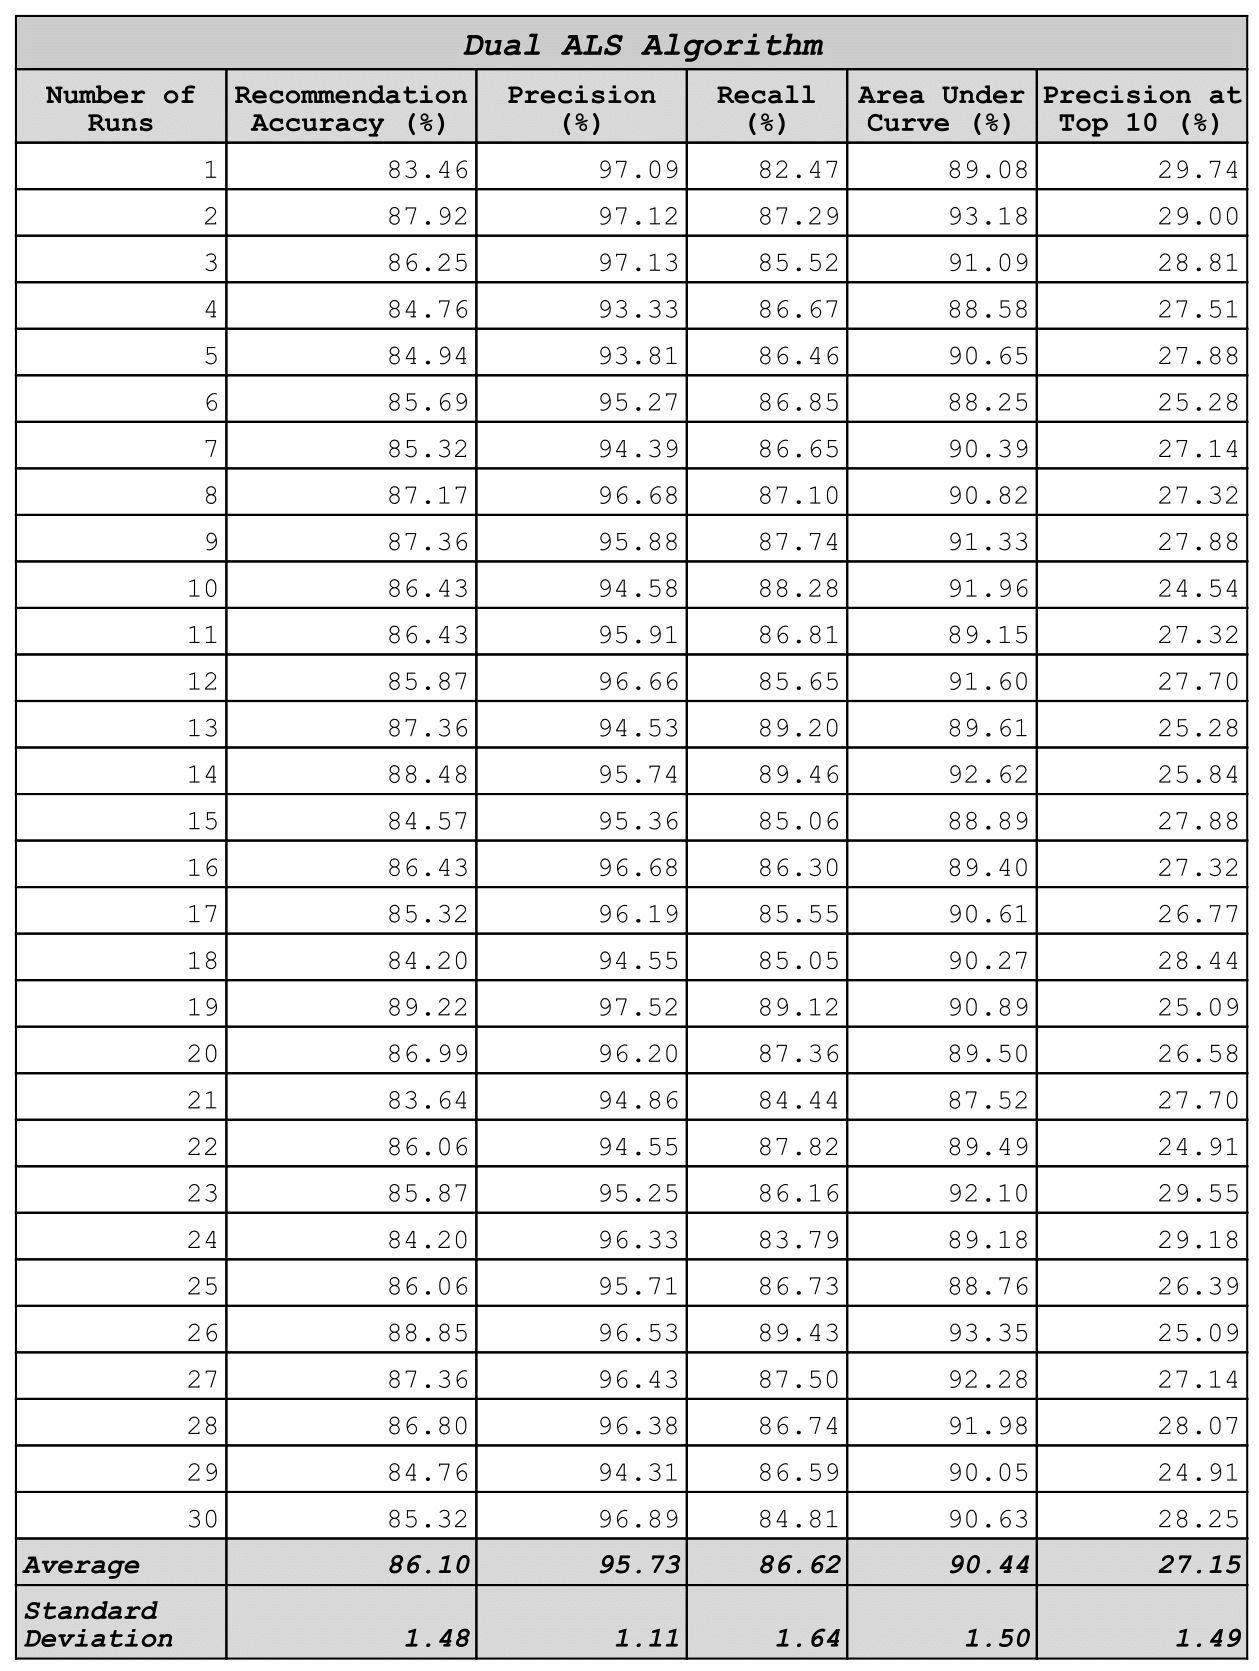
\includegraphics[scale=0.3]{appendices/dual_als_30_runs.png}
\caption{Individual 30 runs of the dual SVD system. }
\label{fig:dual_algorithm}
\end{figure}

\begin{figure}
\centering
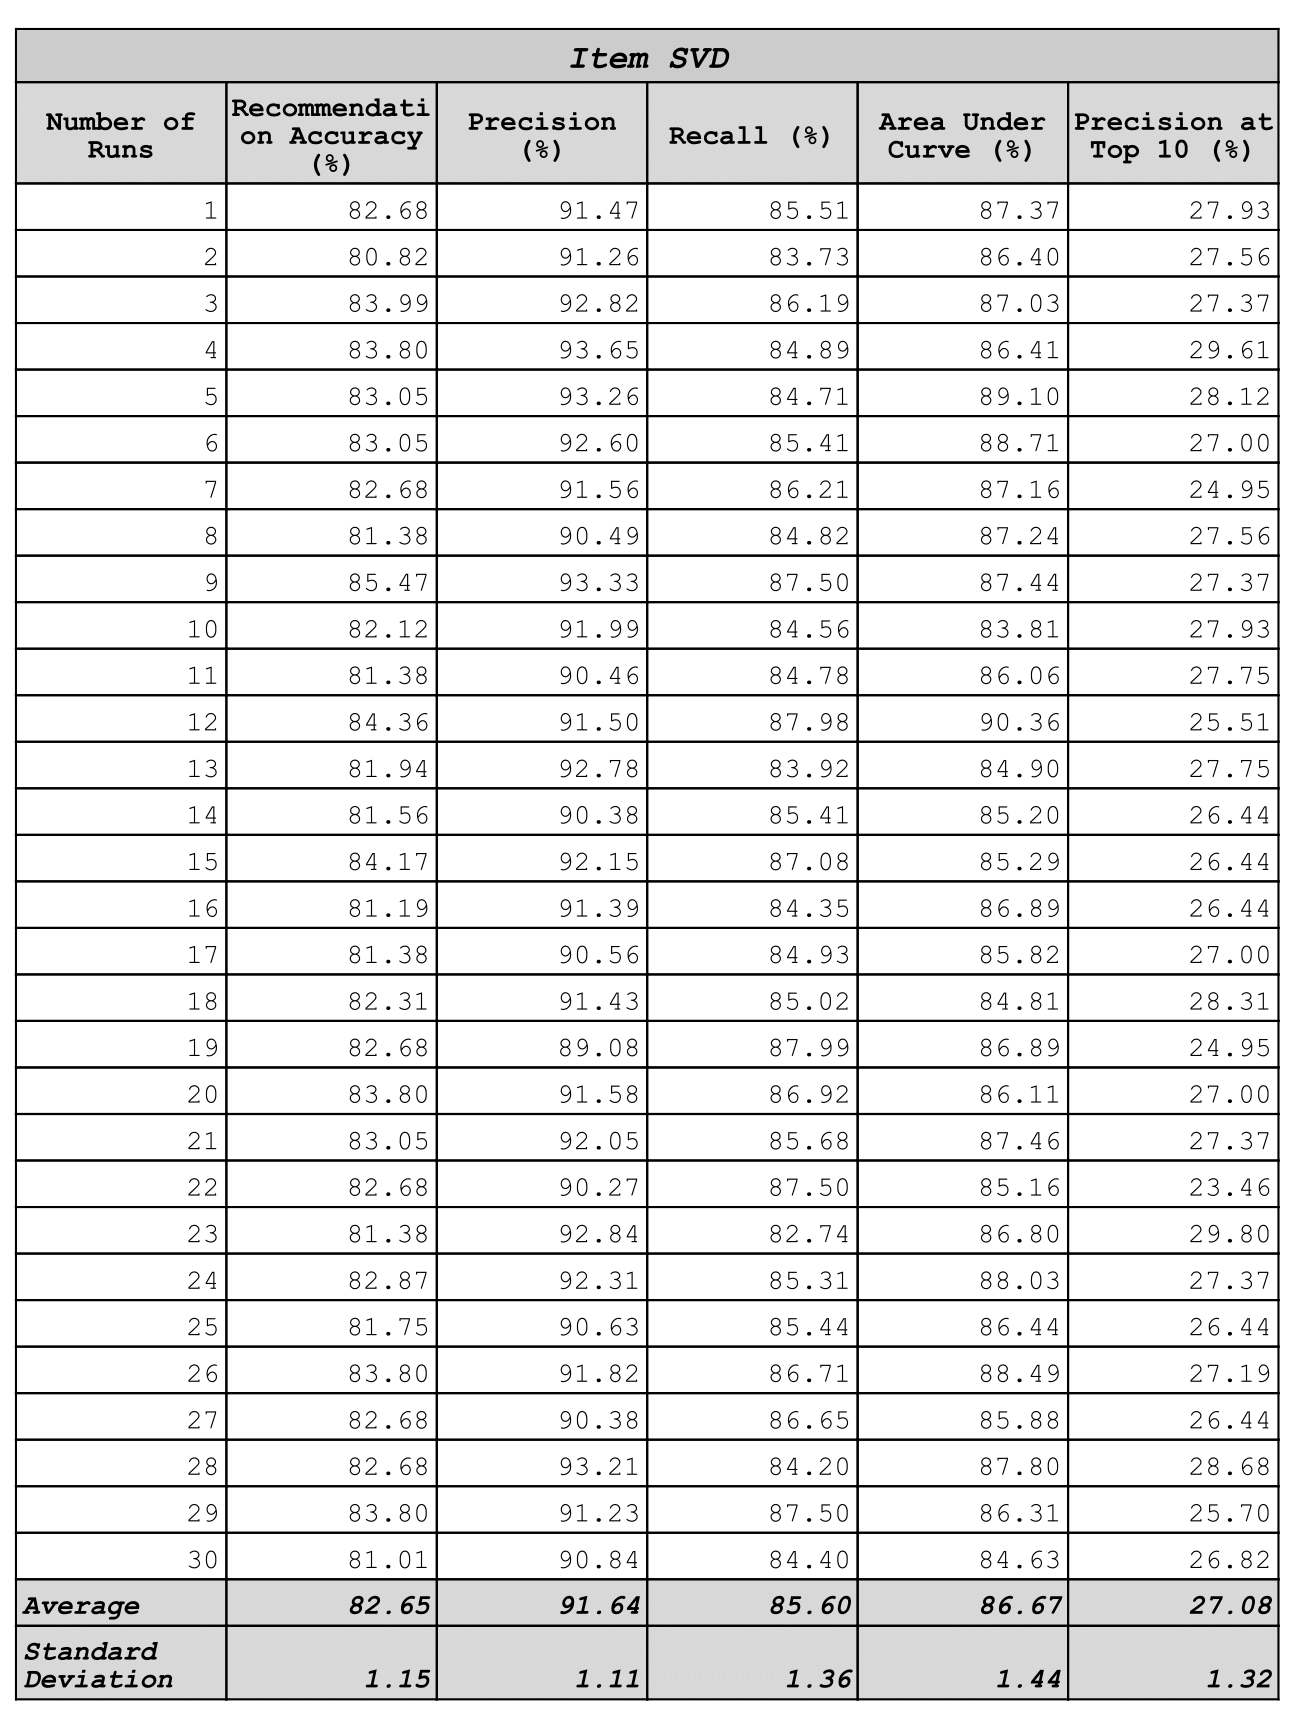
\includegraphics[scale=0.3]{appendices/item_als_30_runs.png}
\caption{Individual 30 runs of the Item SVD system. }
\label{fig:dual_algorithm}
\end{figure}

\begin{figure}
\centering
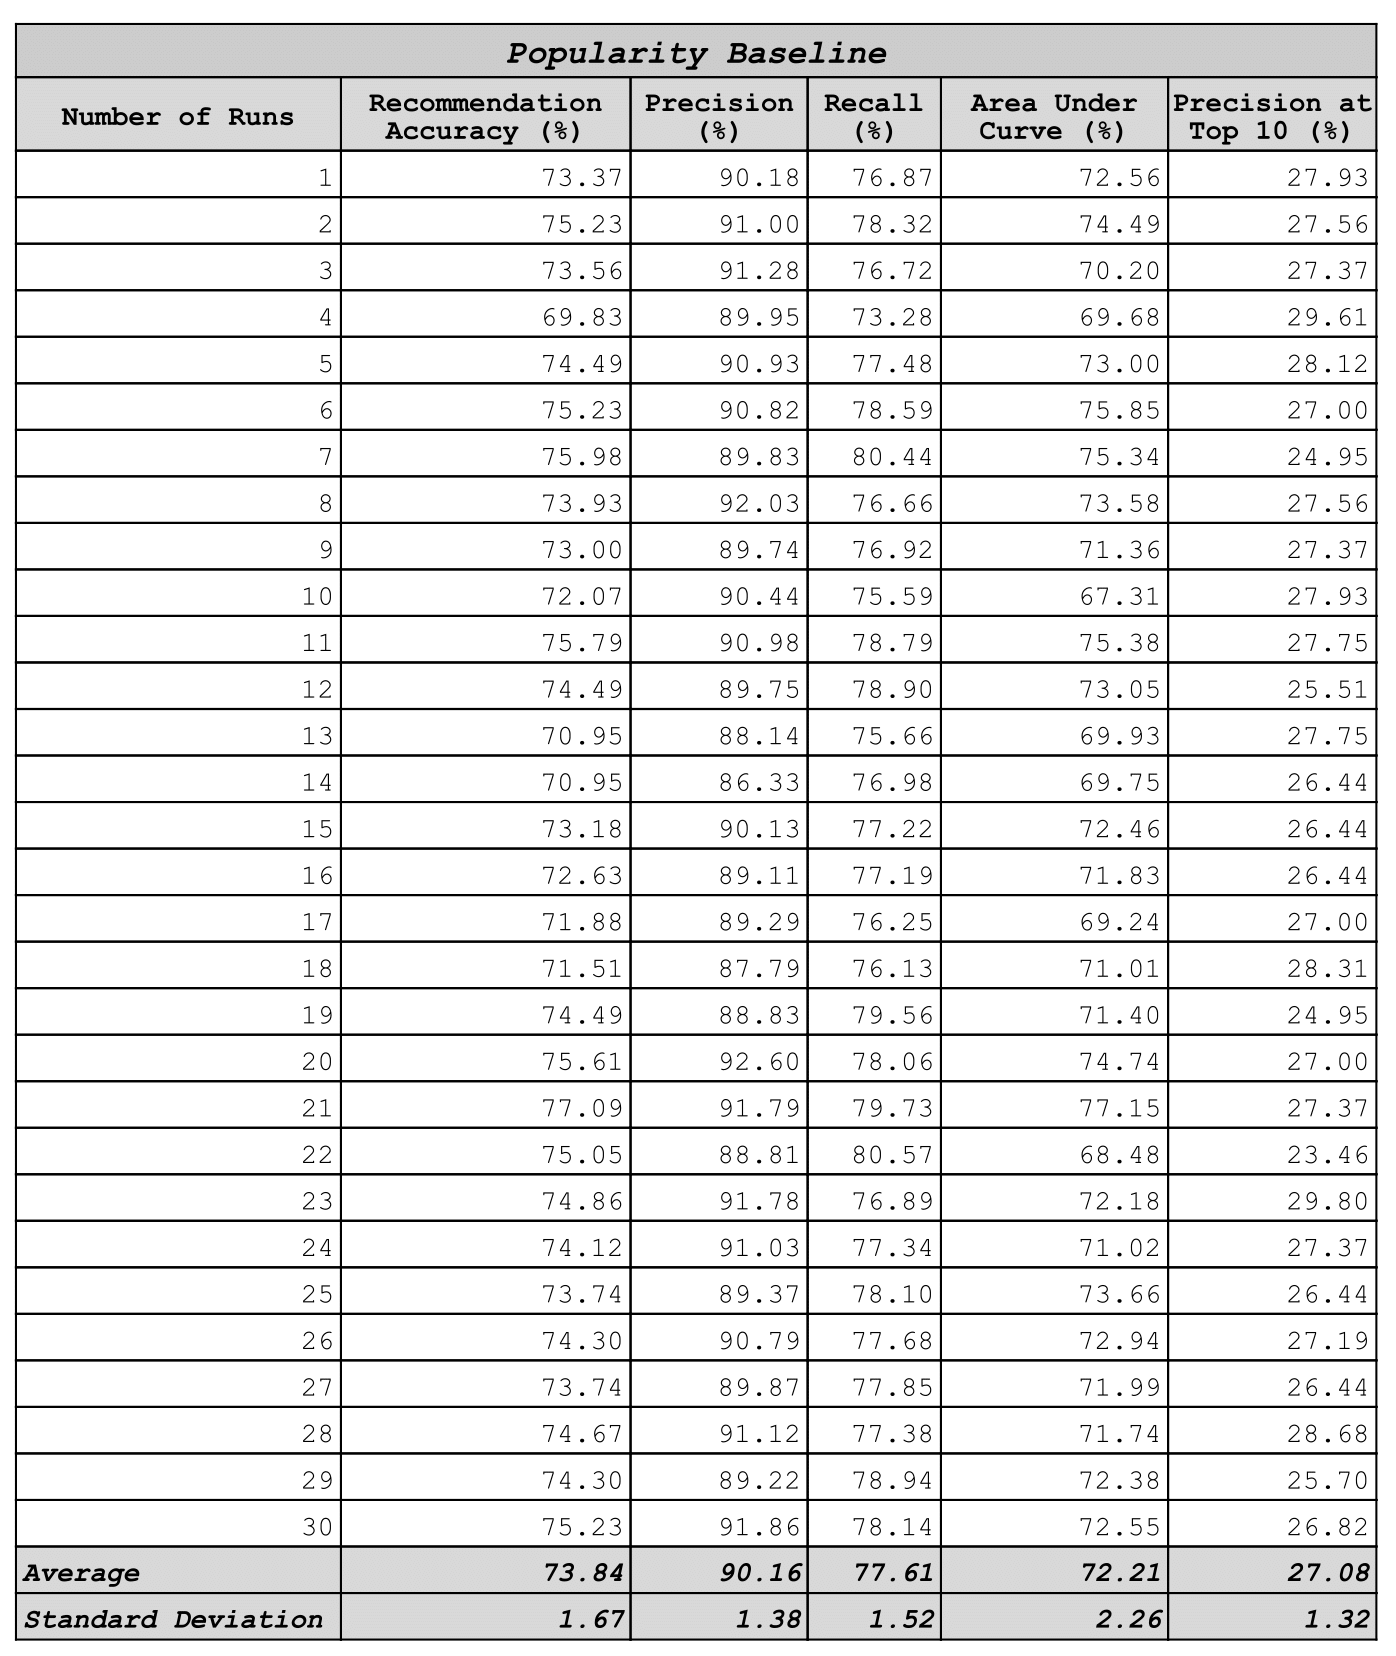
\includegraphics[scale=0.3]{appendices/popular_30_runs.png}
\caption{Individual 30 runs of Baseline Predictor based on item popularity (non-personalised recommendations). }
\label{fig:dual_algorithm}
\end{figure}

\chapter{Survey} \label{appendix:survey}

Contents of the user study. 


\includepdf[pages={1-2}]{appendices/survey_1.pdf}
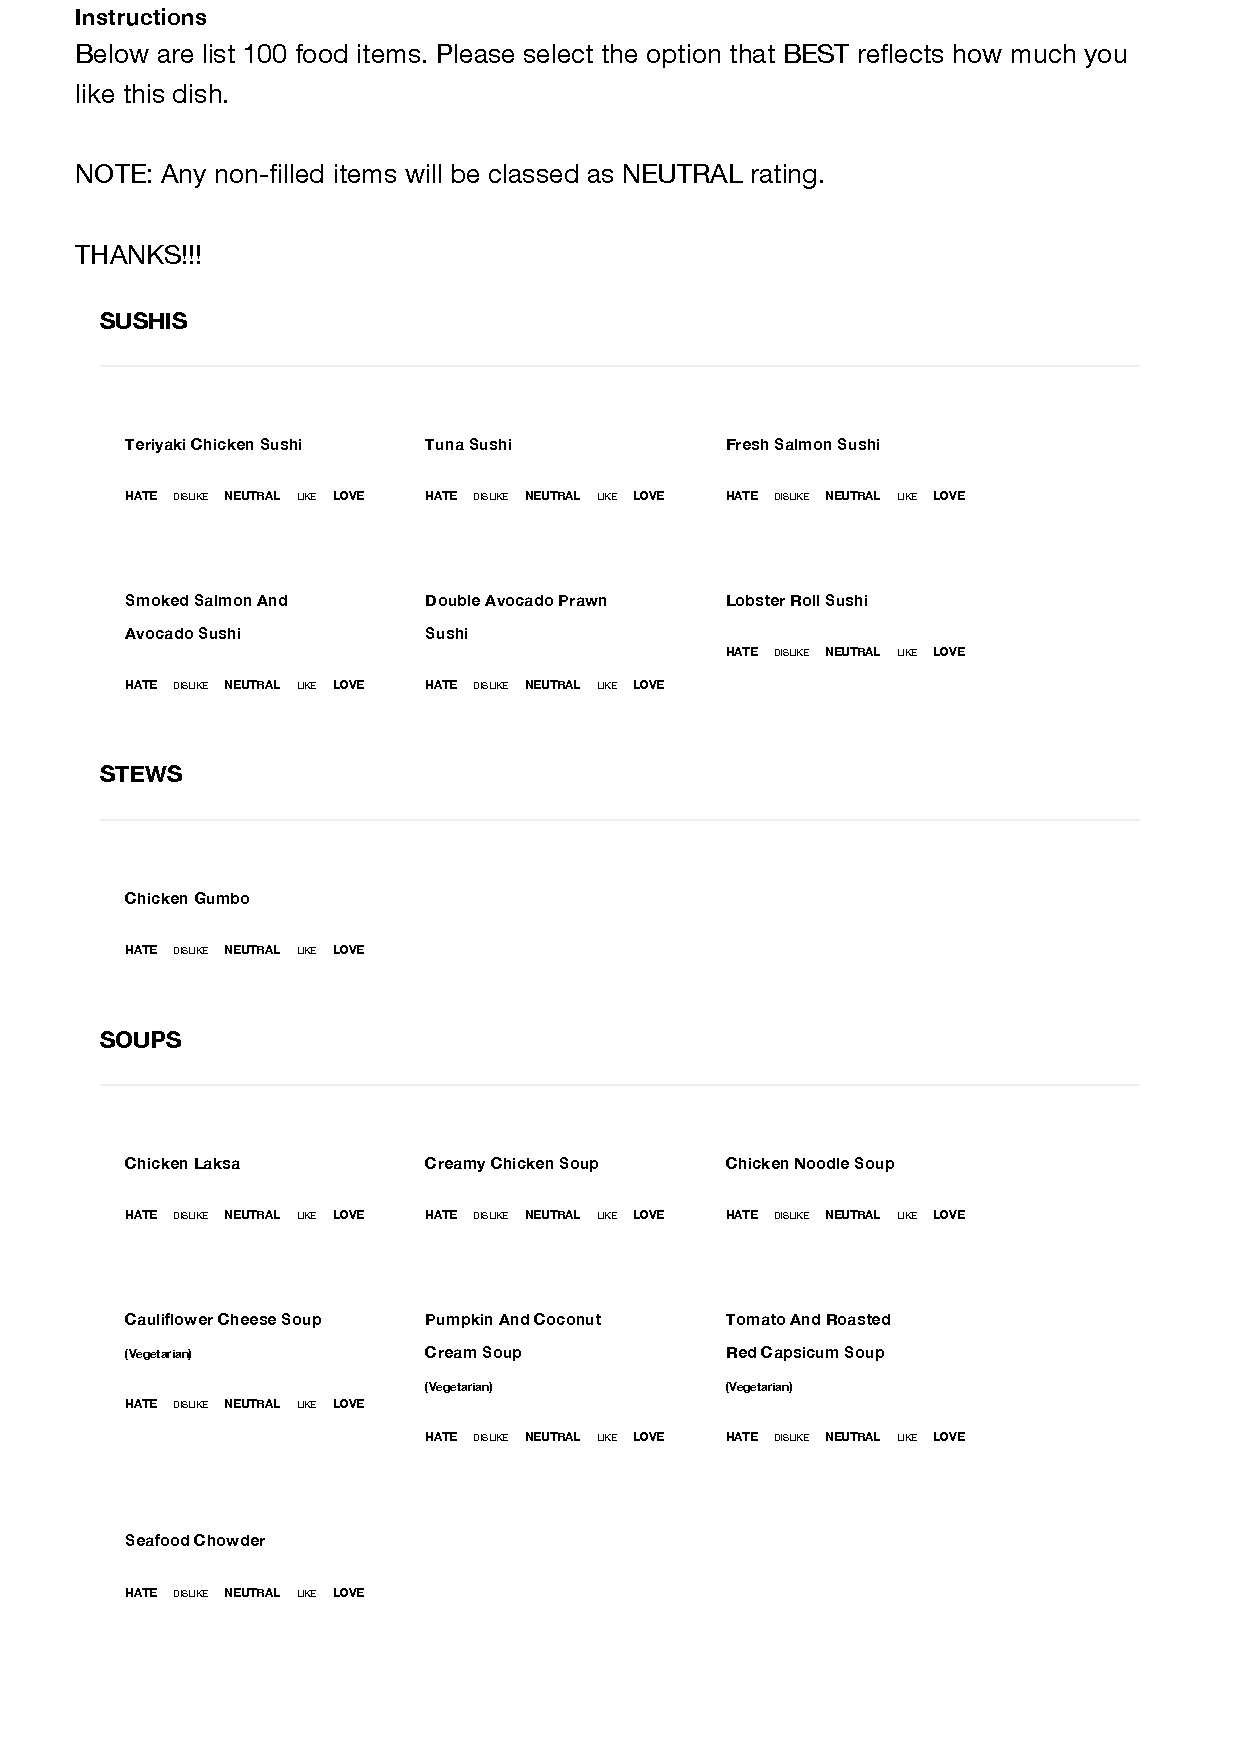
\includepdf[pages={1-7}]{appendices/survey_2.pdf}

\chapter{Human Ethics Committee (HEC)} \label{appendix:hec}

Contents of the Human Ethics Committee, including approval.

\begin{figure} 
\centering

\includegraphics[scale=0.3]{appendices/hec_approval.png}
\caption{Human Ethics Approval for the experiment.}
\label{fig:hec_approval}
\end{figure}


\includepdf[pages={1-2}]{appendices/participant_form.pdf}

\end{appendices}
